\documentclass[12pt, a4paper]{article}

\usepackage[hmargin=2.5cm, vmargin=2cm]{geometry}
\usepackage{amsthm, amssymb, mathtools, yhmath, graphicx}
\usepackage{fontspec, type1cm, titlesec, titling, fancyhdr, tabularx}
\usepackage{color, float, hhline}

\usepackage[abbreviations, per-mode=symbol]{siunitx}
%\usepackage{luatexja-fontspec}
\usepackage[CheckSingle, CJKmath]{xeCJK}
\usepackage{CJKulem}
\usepackage{enumitem}
\usepackage{tikz}
\usepackage{csquotes}
\usepackage{algorithm2e}
\usepackage{circuitikz}
\usepackage{parskip}
\usepackage{bm}
\usepackage{breqn}
\usepackage{mdframed}
\usepackage{bbm}
\usepackage{relsize}
%\setCJKmainfont[BoldFont=cwTex Q Hei]{cwTex Q Ming}
%\setCJKsansfont[BoldFont=cwTex Q Hei]{cwTex Q Ming}
%\setCJKmonofont[BoldFont=cwTex Q Hei]{cwTex Q Ming}
\setCJKmainfont[BoldFont=cwTeX Q Hei]{cwTeX Q Ming}

\def\normalsize{\fontsize{12}{18}\selectfont}
\def\large{\fontsize{14}{21}\selectfont}
\def\Large{\fontsize{16}{24}\selectfont}
\def\LARGE{\fontsize{18}{27}\selectfont}
\def\huge{\fontsize{20}{30}\selectfont}

%\titleformat{\section}{\bf\Large}{\arabic{section}}{24pt}{}
%\titleformat{\subsection}{\large}{\arabic{subsection}.}{12pt}{}
%\titlespacing*{\subsection}{0pt}{0pt}{1.5ex}

\parindent=0pt

\DeclarePairedDelimiter{\abs}{\lvert}{\rvert}
\DeclarePairedDelimiter{\norm}{\lVert}{\rVert}
\DeclarePairedDelimiter{\inpd}{\langle}{\rangle}
\DeclarePairedDelimiter{\ceil}{\lceil}{\rceil}
\DeclarePairedDelimiter{\floor}{\lfloor}{\rfloor}

\DeclareMathOperator*{\argmax}{arg\,max}

\newtheorem{lemma}{Lemma}
\newcommand{\img}{\mathsf{i}}
\newcommand{\ex}{\mathsf{e}}
\newcommand{\dD}{\mathrm{d}}
\newcommand{\dI}{\,\mathrm{d}}
\newcommand{\defeq}{\triangleq}
\DeclareMathOperator{\Expect}{{\rm I\kern-.3em E}}
\DeclareMathOperator*{\ord}{\mathcal{O}}
\providecommand\given{}
% can be useful to refer to this outside \Set
\newcommand*\SetSymbol[1][]{%
  \nonscript\:#1\vert
  \allowbreak
  \nonscript\:
\mathopen{}}
\DeclarePairedDelimiterX\Set[1]\{\}{%
  \renewcommand\given{\SetSymbol[\delimsize]}
  \mkern1mu #1 \mkern1mu
}

\setlength{\droptitle}{-1.5cm} %title 與上緣的間距
\title{Algorithm HW\#2}
\author{B02901178 江誠敏}

\begin{document}
\maketitle
\section{Problem 1.}

First we list some fact that we learned in class: \smallskip

\begin{lemma} \label{lemma:what-we-learn} \hfill
  \begin{enumerate}[label=(\arabic*)]
    \item The commute time $C_{u, v} \defeq h_{u, v} + h_{v, u}$, where
      $h_{u, v}$ is the expected time to walk to $v$ from $u$ could be
      calculated by $C_{u, v} = 2 m R_{u, v}$, where $R_{u, v}$ is
      the effective resistance between node $u, v$ defined in class.
      \label{item:formula-of-commute-time}
    \item For any connected graph, we have $C(G) \leq 2m(n-1)$ where
      $C(G) \defeq \max C_u(G)$ and $C_u(G)$ is the expected
      time to traverse from $u$ to all other states.
      Tracing the proof given in class we also have a
      modified bound $C(G) \leq 2 m R_{u, v}$.
      \label{item:bound-of-cover-time}
  \end{enumerate}
\end{lemma}

Now, for the lower bound, notice that $C_u(G) \geq \max_v h_{u, v}$
by definition. Also $2 m R_{u, v} = C_{u, v} = h_{u, v} + h_{v, u}$
by \ref{item:formula-of-commute-time} of lemma~\ref{lemma:what-we-learn},
which implies one of the $h_{u, v}, h_{v, u}$ is no less than
$2 m R_{u, v} / 2 = m R_{u, v}$, thus
\[ C(G) = \max C_u(G) \geq \max h_{u, v} \geq \max \,\Set{ m R_{u, v} } = m R(G) \]

For the upper bound, again
by \ref{item:formula-of-commute-time} of lemma~\ref{lemma:what-we-learn},
\[ h_{u, v} \leq C_{u, v} = 2m R_{u, v} \leq 2 m R(G) \]

Now, for a random walk started from $u$,
we shall calculate the probability of a vertex $v$ that has not been visited
after $16 m R(G)$ steps. Recall Markov inequality: \smallskip
\begin{lemma}[Markov]
  If $X$ is a random variable with $\Pr\Set{ X \geq 0 } = 1$, then
  \[ \Pr \Set{X \geq \alpha \Expect X} \leq 1 / \alpha \]
\end{lemma}
Since the expectation time to walk to $v$ from $u$ is $h_{u, v} \leq 2 m R(G)$,
the propability $\Pr\Set{ v \text{ not visited}} \leq 2 m R(G) / (16 m R(G)) = 2^{-3}$.

Now, after $16 m R(G)$ steps, assume we end up in vertex $u'$, and $v$ has not been visited.
We continue a walk of $16 m R(G)$ steps from $u'$, and again the probability
of $v$ not been visited in this walk is $2^{-3}$. If we repeat the process
for $\log_2 n$ times, we have
\[ \Pr\Set{ v \text{ not visited among these} \log_2 n \text{ walks} } \leq (2^{-3})^{\log_2 n} = n^{-3} \]
Thus by union bound, if $p$ is the probability that exists a vertex $v$ not visited after
$16 m R(G) \log_2 n$ steps, then $p \leq n^{-3} \cdot n = n^{-2}$.

If we haven't visited all the vertex after $16 m R(G) \log_2 n$ steps,
and assume we are at vertex $u$. Forget about the previous walk and regard
the walk afterward as a new random walk started from vertex $u$,
then using the modified bound mentioned in
\ref{item:bound-of-cover-time} of lemma~\ref{lemma:what-we-learn},
the expected time to walk through all the vertex is bounded by $2 m R(G) (n-1) \leq 2mn$,
thus the expected time from the very begining is bounded by
\begin{align*}
  & (1-p) 16 m R(G) \log_2 n + p ( 16 m R(G) \log_2 n + 2m R(G) n) \\
  & \leq 16 m R(G) \log_2 n + 2mR(G)/n \\
  & \leq 32 m R(G) \log_2 n
\end{align*}
since $1/n \leq \log_2 n$.

If we could assume $G$ is a simple graph, then another way to bound the expectation
is to consider $32 m R(G) \log_2 n$ step instead of $16 m R(G) \log_2 n$ steps,
and thus $p \leq n^{-3}$, so
using the original bound in \ref{item:bound-of-cover-time} of lemma~\ref{lemma:what-we-learn},
\begin{align*}
  & (1-p) 32 m R(G) \log_2 n + p ( 32 m R(G) \log_2 n + 2m n) \\
  & \leq 16 m R(G) \log_2 n + 2m/n^2 \\
  & \leq 32 m R(G) \log_2 n + 1
\end{align*}
since $m \leq n^2 / 2$ now.

{\bf Collaborators}: None.

\section{Problem 2.}
Follow the hint, first we prove a lemma: \smallskip
\begin{lemma}
  Each flip in the algorithm decreases the difference with probability at least $1/2$.

  \begin{proof}
    Without loss of generality, assume the clause is $(x_1 \lor x_2)$.
    Since the clause is not satisfied before flipping, both $x_1$ and $x_2$
    are \texttt{False}, and in the satisfying assignment, at least one of
    them are \texttt{True}, which is choosed to flip with probability
    at least $1/2$.
    Other situation (e.g., $\lnot x_1 \lor x_2$) follows similarly.
  \end{proof}
\end{lemma}

Now, let $u_k, \, 0 \leq k \leq n$ be the state such that the difference between the current assignment
and the satisfying assignment is $k$, and $P(u_k, u_h)$ be the transition probability
of two states, then $u_k$ only transit to state $u_{k+1}, u_{k-1}$ and
$P(u_k, u_{k-1}) \geq 1/2$ by the lemma above.
What we want is a bound of $E(u_k, u_0)$, the expected time to walk from $u_k$ to $u_0$.

Consider the following undirected graph Markov chain:
\begin{figure}[H]
  \centering
  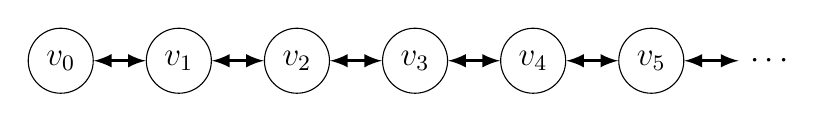
\begin{tikzpicture}
    \tikzstyle{nd}=[draw, circle]
    \foreach \x in {0, 1, ..., 5}
      \node[nd] (\x) at ({1.5*\x}, 0) {$v_\x$};
    \node (6) at (9, 0) {$\cdots$};
    \foreach \x [count=\xi from 1] in {0, 1, ..., 5}
      \draw[very thick, latex-latex] (\x) -- (\xi);
  \end{tikzpicture}
\end{figure}
Which $P(v_k, v_{k-1}) = 1/2 \leq P(u_k, u_{k-1})$ for $k \geq 1$,
so we must have $E(v_k, v_0) \geq E(u_k, u_0)$.
Now by \ref{item:formula-of-commute-time} of lemma~\ref{lemma:what-we-learn},
$E(v_n, v_0) + E(v_0, v_n) = 2 m R(v_k, v_0) = 2 mk \leq 2 n^2$ since the number of edge $m$
is equal $n$ by the fact that there are $n+1$ nodes.
By symmetry, $E(v_0, v_n) = E(v_n, v_0)$, so $E(v_n, v_0) = n^2$.
Also we have $E(v_n, v_0) \geq E(v_k, v_0)$ since the path
from $v_n$ to $v_0$ must go through $v_k$, so $E(v_n, v_0) = E(v_n, v_k) + E(v_k, v_0)$.
Hence $E(u_k, u_0) \leq E(v_k, v_0) \leq E(v_n, v_0) \leq n^2$.

Using a similar argument in problem 1., consider a random walk with $2n^2 \log_2 n$
steps, divide into $\log_2 n$ section with $2 n^2$ steps each.
Each section could be regard as a random walk started at some vertex $u_k$,
thus by Markov inequality, $u_0$ is not visited in this section
has probability less then $n^2 / (2 n^2) = 1/2$, so the probability
such that $u_0$ is not visited in $2 n^2 \log_2 n$ steps is no more then
$(1/2)^{\log_2 n} = 1/n$, thus the algorithm finds a satisfying
assignment with probability at least $1 - 1/n$.

{\bf Collaborators}: None.

\section{Problem 3.}
As hint, repeat $A$ $m$ times and get $m$ estimations $a_1, \dots, a_m$.
Let $a$ be the median of $a_i$, $R, L = (1 \pm \epsilon) \#(I)$,
then if $\# \Set{i : a_i < L} < m/2$
and $\# \Set{i: a_i > R} < m/2$ both hold, we must have $L \leq a \leq R$.
Since $\Pr\Set{L \leq a_i \leq R} \geq 3/4$, we have $\Pr\Set{a_i < L} \leq 1/4$.
Now, let $X_i = 1$ if $a_i < L$, or else $0$, then $\Pr\Set{X_i = 1} \leq 1/4$ and
each $X_i$ are independent Bernoulli random variable.
Let $X = \sum X_i$, we have
\[ \Pr\Set*{\# \Set{i: a_i < L} \geq \frac{m}{2} } = \Pr\Set*{ X \geq \frac{m}{2} } \]

Recall Chernoff bound: \smallskip
\begin{lemma}
  If $X_1, \dots, X_m$ are independent Bernoulli random variable and $X = \sum X_i$,
  $\mu = \Expect X$, then
  $\Pr\Set{X \geq \mu + \lambda} \leq \exp\left( \frac{-2\lambda^2}{m} \right)$.
\end{lemma}

Now, $\mu \defeq \Expect X \leq m/4$, so
\[ \Pr\Set*{X \geq \frac{m}{2}} = \Pr\Set*{X \geq \mu + \frac{m}{2} - \mu}
  \leq \exp\left( \frac{- 2 (m/4)^2}{m} \right) \leq \exp\left( \frac{-m}{8} \right) \]
since $m/2 - \mu \geq m/4$. If we let $m = 8 \log(2\delta)$ which is polynomial in $\log \delta$,
then
\[ \Pr\Set*{\# \Set{i: a_i < L} \geq \frac{m}{2} } =
 \Pr\Set*{X \geq \frac{m}{2}} \leq \frac{1}{2 \delta} \]
Similarly,
\[ \Pr\Set*{\# \Set{i: a_i > R} \geq \frac{m}{2} } \leq \frac{1}{2 \delta} \]
By the union bound,
\begin{align*}
  & \Pr\Set{L \leq a \leq R} \\
  & = 1 - \Pr\Set*{\# \Set{i: a_i < L} \geq \frac{m}{2}
    \ \text{ and }\  \# \Set{i: a_i > R} \geq \frac{m}{2} } \\
  & \leq \frac{1}{2 \delta} + \frac{1}{2 \delta} = 1 - \frac{1}{\delta}
\end{align*}
Since $A$ is an algorithm with running time polynomial in $n, \epsilon^{-1}$,
and we repeat $A$ $m$ times, which is polynomial in $\log \delta^{-1}$,
the overall running time is polynomial in $n, \epsilon^{-1}, \log \delta^{-1}$.

{\bf Collaborators}: None.

\section{Problem 4.}

First we consider the probabilistic sampling problem:

Given an universe $U$, which each $x \in U$ appears with probability $p(x)$.
Given $G \subseteq U$, Estimate $P \defeq \sum_{x \in G} p(x)$.

This problem could be solved using a similar algorithm:

\begin{enumerate}
  \item Sample $n$ samples $X_1, \dots, X_n$ by $p$.
  \item Let $Y = \sum_{i} \raisebox{-.05em}{$\mathlarger{\mathbbm{1}}$}[ X_i \in G ]$,
    output $\hat{P} \defeq Y/n$.
\end{enumerate}

We have similar result to the original version. \smallskip

\begin{lemma} \label{lemma:modified-sampling}
  If we pick $n \geq 3 \log(2/\delta) / (\epsilon^2 P)$, then
  $ \Pr\Set*{ \abs{\hat{P} - P} \leq \epsilon P } \geq 1 - \delta $.

  \begin{proof}
    Let $Y_i = \raisebox{-.05em}{$\mathlarger{\mathbbm{1}}$}[ X_i \in G ]$,
    then $Y = \sum Y_i$ and $\Expect Y_i = P$ implies that $\Expect Y = nP$.
    So
    \begin{align*}
      \Pr\Set*{ \abs{\hat{P} - P} \leq \epsilon P } &=
      \Pr\Set{\abs{Y - \Expect Y} \leq \epsilon \Expect Y} \\
      &= 1 - \Pr\Set{\abs{Y - \Expect Y} \geq \epsilon \Expect Y} \\
      &\stackrel{(a)}{=} 1 - 2 \exp\left( \frac{-\epsilon^2 \Expect Y}{3} \right) \\
      &\geq 1 - 2 \exp( -\log(2/\delta) ) = 1 - \delta
    \end{align*}
    Where (a) is because of Chernoff bound.
  \end{proof}
\end{lemma}

Now, as in the original DNF counting problem, let $\mathcal{I}$ be all
the possible assignment (since there are $n$ variables, $\abs{\mathcal{I}} = 2^n$),
$\mathcal{J} = \Set{1, \dots, m}$ be the indices of all clauses,
and define $U \subseteq \mathcal{I} \times \mathcal{J}$ by
$U \defeq \Set{ (\alpha, j) : \text{assignment } \alpha \text{ satisfies } j\text{th clause}}$,
Each $(\alpha, j) \in U$ has probability $p((\alpha, j)) = C p(\alpha)$,
where $C$ is a normalizing factor, and $p(\alpha)$ is the probability of assignment $\alpha$.
That is, if $\alpha$ is the assignment that set $x_i : i \in A$ to \texttt{True},
then $p(\alpha) = \prod_{i \in A} p_i \cdot \prod_{i \not\in A} (1 - p_i)$.

Define $U = \Set{(\alpha, j) : j \text{ is the smallest s.t. } (\alpha, j) \in U}$,
then the probability of the DNF be satisfied is $C^{-1} \sum_{(\alpha, j) \in U} p((\alpha, j))$.
Notice that
\[ 1 = \sum_{(\alpha, i) \in U} p((\alpha, i))
  = \sum_{(\alpha, j) \in G} \sum_{i: (\alpha, i) \in U} p((\alpha, i))
  \leq \sum_{(\alpha, j) \in G} m \cdot p((\alpha, j)) \]
So $q \defeq \sum_{(\alpha, j) \in G} p((\alpha, j)) \geq 1 / m$.
By using the probabilistic sampling algorithm with lemma~\ref{lemma:modified-sampling},
we have an estimate $\hat{q}$ of $q$ such that $\Pr\Set{\abs{\hat{q} - q} \leq \epsilon q} \geq 1 - \delta$,
which only need $\ord(m \log(\delta^{-1}) / \epsilon^2$ samplings.

Now, we shall guarantee that sampling from $U$ uniformly could be achieve in polynomial time.
First define $P_j \defeq \sum_{\alpha: (\alpha, j) \in U} p(\alpha)$, which is the sum
of probability of those assignments which satisfy $j$-th clause. Define
\begin{align*}
  A &= \Set{ i: x_i \text{ appears in the clause}} \\
  B &= \Set{ i: \lnot x_i \text{ appears in the clause}} \\
  C &= \Set{ i: \text{both } x_i \text{ and } \lnot x_i \text{ does not appear in the clause}}
\end{align*}
We could assume that $A \cap B = \varnothing$, or else the clause could never be satisfied.
Then it is easy to see that if an assignment satisfy the clause,
then $x_i : i \in A$ must be set to \texttt{True}, and $x_i : i \in B$ must be
set to \texttt{False}, while the remains (i.e., $x_i : i \in C$) could
be set to either one. Therefore the total probability is
\[ P_j = \prod_{i \in A} p_i \cdot \prod_{i \in B} (1 - p_i) \]
which could be compute easily. Knowing $P_i$, $C = (\sum P_j)^{-1}$ could be calculated.

Finally, to sample $(\alpha, j)$ based on distribution $p((\alpha, j))$, we could
first sample $j$ by $C P_j$, and then sample an $(\alpha, j) \in U$ with probability
$p((\alpha, j)) / (C P_j) = p(\alpha) / P_j$. The last step is simple,
just randomly set $x_i : i \in C$ to be \texttt{True} with probability $p$
and \texttt{False} with probability $1-p$ while each $x_i : i \in A$
set to \texttt{True} and $x_i : i \in B$ set to \texttt{False}.

The process mentioned above runs in polynomial of $n, m$, where $n$ is
the number of variables and $m$ is the number of clauses, are all
polynomial to the input size. The sampling algorithm
runs in polynomial of $m, \log(\delta^{-1}), \epsilon^{-1}$,
thus the overall algorithm is an RFTAS.

{\bf Collaborators}: None.

\end{document}

